\documentclass[chappg, 12pt,a4paper, hidelinks, oneside]{memoir}
% \documentclass[titlepage,12pt,a4paper]{book}

% substituir linha seguinte por 
% \usepackage[english]{babel} 
% se o relatório for escrito na língua inglesa.
\usepackage[portuguese]{babel}

\usepackage[utf8]{inputenc}
\usepackage{makeidx}
\usepackage{xspace}
\usepackage{graphicx,color,times}
\usepackage{fancyhdr}
\usepackage{pxfonts}
\usepackage{times}
\usepackage{amssymb}
\usepackage{amsfonts}
\usepackage{latexsym}
\usepackage[printonlyused]{acronym}
\usepackage{float}
\usepackage{listings}
\usepackage{tocbibind}
\usepackage{natbib}
\usepackage{hyperref}
\usepackage[T1]{fontenc}
\usepackage{titlesec, blindtext, color}
\usepackage{courier}
\usepackage{fix-cm}
\usepackage{fourier}
\usepackage[scaled=.92]{helvet}
\usepackage{geometry}
\usepackage{floatrow}

% \usepackage{glossaries}
% \makeglossaries

% \renewcommand{\ttdefault}{phv}

\pagestyle{fancy}
\renewcommand{\chaptermark}[1]{\markboth{#1}{}}
\renewcommand{\sectionmark}[1]{\markright{\thesection\ #1}}
\fancyhf{} \fancyhead[L,RO]{\bfseries\thepage}
\fancyhead[LO]{\bfseries\rightmark}
\fancyhead[R]{\bfseries\leftmark}
\renewcommand{\headrulewidth}{0.5pt}
\renewcommand{\footrulewidth}{0pt}
\setlength{\headheight}{15.6pt}
\setlength{\marginparsep}{0cm}
\setlength{\marginparwidth}{0cm}
\setlength{\marginparpush}{0cm}
\addtolength{\hoffset}{-1.0cm}
\addtolength{\oddsidemargin}{\evensidemargin}
\addtolength{\oddsidemargin}{0.5cm}
\addtolength{\evensidemargin}{0.5cm}

\titleformat{\chapter}[hang]
    {\Huge\bfseries}{\thechapter\hspace{0.75cm}\hsp\textcolor{gray75}{/}\hspace{0.75cm}}{0pt}{\Huge\bfseries\slshape}
    \titlespacing*{\chapter}{0pt}{-10pt}{20pt}
\titleformat{\section}[hang]
    {\Large\bfseries}{\thesection\hspace{0.5cm}\textcolor{gray75}{|}\hspace{0.5cm}}{0pt}{\Large\bfseries}
\titleformat{\subsection}[hang]
    {\large\bfseries}{\thesubsection\hspace{0.2cm}\textcolor{gray75}{-}\hspace{0.2cm}}{0pt}{\large\bfseries}


\usepackage{fix-cm}
\usepackage{fourier}
\usepackage[scaled=.92]{helvet}
\definecolor{ChapGrey}{rgb}{0.6,0.6,0.6}
\newcommand{\LargeFont}{
  \usefont{\encodingdefault}{\rmdefault}{b}{n}
  \fontsize{60}{80}\selectfont\color{ChapGrey}
  }
\makeatletter
\makechapterstyle{GreyNum}{
  \renewcommand{\chapnamefont}{\large\sffamily\bfseries\itshape}
  \renewcommand{\chapnumfont}{\LargeFont}
  \renewcommand{\chaptitlefont}{\Huge\sffamily\bfseries\itshape}
  \setlength{\beforechapskip}{-20pt}
  \setlength{\midchapskip}{-20pt}
  \setlength{\afterchapskip}{-60pt}
  \renewcommand\chapterheadstart{\vspace*{\beforechapskip}}
  \renewcommand\printchaptername{
  \begin{tabular}{@{}c@{}}
    \chapnamefont \@chapapp\\}
    \renewcommand\chapternamenum{\noalign{\vskip 2ex}}
    \renewcommand\printchapternum{\chapnumfont\thechapter\par}
    \renewcommand\afterchapternum{
  \end{tabular}
  \par\nobreak\vskip\midchapskip}
  \renewcommand\printchapternonum{}
  \renewcommand\printchaptertitle[1]{
  {\chaptitlefont{##1}\par}}
  \renewcommand\afterchaptertitle{\par\nobreak\vskip \afterchapskip}
}
\makeatother
\chapterstyle{GreyNum}

\setcounter{tocdepth}{3}
\setcounter{secnumdepth}{3}
\setsecnumdepth{subsubsection}

\renewcommand{\ttdefault}{lmtt}


% NEW COLORS
\definecolor{gray75}{gray}{0.75}
\definecolor{dark}{gray}{0.25}
\definecolor{lgray}{gray}{0.9}
\definecolor{dkblue}{rgb}{0,0.13,0.4}
\definecolor{dkgreen}{rgb}{0,0.6,0}
\definecolor{gray}{rgb}{0.5,0.5,0.5}
\definecolor{mauve}{rgb}{0.58,0,0.82}


\usepackage{caption}
\DeclareCaptionFont{white}{\color{white}}
\DeclareCaptionFormat{listing}{\colorbox{gray}{\parbox{\textwidth}{#1#2#3}}}
\captionsetup[lstlisting]{format=listing,labelfont=white,textfont=white}


\lstdefinestyle{Cpp} {
language=C,
basicstyle=\small\sffamily,
numbers=left,
numberstyle=\tiny,
columns=fullflexible,
showstringspaces=false
xleftmargin=-10pt,
xrightmargin=-10pt,
}

\renewcommand{\lstlistingname}{Excerto de Código}
\renewcommand{\lstlistlistingname}{Lista de Excertos de Código}

\renewcommand{\today}{\day \ifcase \month \or Janeiro\or Fevereiro\or Março\or %
Abril\or Maio\or Junho\or Julho\or Agosto\or Setembro\or Outubro\or Novembro\or %
Dezembro\fi de \number \year} 

% Custom command for empty page between chapters
\newcommand{\emptypage}{
    \null
    \thispagestyle{empty}
    \clearpage
}

\begin{document}


\thispagestyle{empty}
\setcounter{page}{-1}

\begin{center}
\begin{Huge}
\textbf{Universidade da Beira Interior}
\end{Huge}
\end{center}

\begin{center}
\begin{Huge}
Licenciatura em Engenharia Informática
\end{Huge}
\end{center}

\vspace{0,07cm}
\begin{figure}[!htb]
\centering
\includegraphics[width=191pt]{ubi-fe-di.png}
\end{figure}

\vspace{0.5cm}
\begin{center}
\begin{Large}
\textbf{\emph{Sistema Solar}}
\end{Large}
\end{center}


\vspace{0.15cm}
\begin{center}
\begin{normalsize}
\begin{large}
Elaborado por:
\end{large}
\end{normalsize}
\end{center}

\vspace{0.005cm}
\begin{center}
\textbf{António Cruz, 47995} \\
\textbf{Francisco Santos, 47711} \\
\textbf{Leonardo Santos, 48708} \\
\textbf{Ruben Carvalho, 46180}
\end{center}



\vspace{0.15cm}
\begin{center}
\begin{normalsize}
\begin{large}
Orientador:
\end{large}
\end{normalsize}
\end{center}

\vspace{0.05cm}
\begin{center}
\begin{large}
  \textbf{Professor Doutor Abel Gomes}
\end{large}
\end{center}

\vspace{0.15cm}
\begin{center}
\begin{normalsize}
\begin{large}
Unidade Curricular:
\end{large}
\end{normalsize}
\end{center}

\vspace{0.05cm}
\begin{center}
\begin{large}
\textbf{Computação Gráfica}
\end{large}
\end{center}

\vspace{0.05cm}
\begin{center}
\begin{normalsize}
\today, Covilhã
\end{normalsize}
\end{center}


\frontmatter

\emptypage
\chapter*{Agradecimentos}
\label{chap:ack}
\vspace{0.7cm}

Após terminar o projeto, é impossível não refletir sobre a imensa contribuição que recebemos ao longo do tempo. Neste capítulo, gostaríamos de expressar os nossos mais profundos 
agradecimentos ao professor Abel João Padrão Gomes e a todos os membros do grupo que tornaram esta experiência educacional significativa. Ao professor, expressamos a nossa mais sincera gratidão. O seu comprometimento apaixonado com o ensino e a sua dedicação incansável ao compartilhamento de conhecimento foram fundamentais para o nosso aprendizado. Além disso, não podemos deixar de expressar nossa gratidão a cada membro do grupo. Cada um de nós trouxe uma perspectiva única, habilidades distintas e um compromisso inabalável com a realização dos objetivos do trabalho.
As nossas reuniões foram marcadas por colaboração, criatividade e respeito mútuo, elementos essenciais para o nosso sucesso coletivo. A troca de ideias, o trabalho árduo e a camaradagem que cultivámos juntos foram fundamentais para enfrentar os desafios que encontrámos ao longo deste percurso académico. Cada membro do grupo desempenhou um papel vital, contribuindo não apenas para a conclusão do trabalho, mas também para o crescimento individual de cada um. É impossível deixar de agradecer também aos nossos familiares, que se fizeram presentes, nos dias bons e maus, e em momento algum nos deixaram cair, apoiando-nos sempre para nos mantermos no bom sentido, nesta que é a nossa caminhada para o sucesso profissional.

\chapter*{Resumo}
\label{chap:res}
\vspace{0.7cm}

Pensar que cada ser humano é apenas uma peça pequena de um grande puzzle que constitui a nossa galáxia deixa muitas pessoas fascinadas, pela nossa inferioridade comparando com a complexidade e o tamanho do que nos rodeia. Para essas pessoas é ainda mais fascinante ver os elementos do sistema solar com os seus próprios olhos, com ajuda de telescópios e imagens partilhadas por satélites, apesar de nem sempre ser fácil de conseguir ver o que queremos. Mas e se conseguissemos representar o nosso sistema solar num computador? Seria muito mais fácil e barato ver tudo aquilo que queremos, sem saírmos das nossas próprias casas, para além de nos fornecer uma maior imersão.
Ao longo deste documento vamos explicar detalhadamente como foi desenvolvida e implementada a nossa versão do sistema solar, com os vários planetas e informações sobre os mesmos. Vamos explicar também a magia que fez todas as físicas dos planetas funcionar, como utilizámos bibliotecas de \ac{UI} para criar menus que possibilitam alterar partes do sistema em tempo real, e muito mais.


\emptypage
\chapter*{Acrónimos}
\label{chap:acro}

% #   ATENÇÃO
% A lista de acrónimods deve ser ordenada alfanumericamente.
% Estrangeirismos devem ser realçados em itálico.
% Se o relatório for escrito em Inglês, uma palavra portuguesa é um estrangeirismo.

% O maior acrónimo deve ser colocado neste ponto.
%               vvvvvv
\begin{acronym}[IMGUI]

  \acro{CG}{Computação Gráfica}
  \acro{GPU}{\textit{Graphics Processing Unit}}
  \acro{HDR}{\textit{High Dynamic Range}}
  \acro{IMGUI}{\textit{Immediate Mode Graphic User Interface}}
  \acro{LDR}{\textit{Low Dynamic Range}}
  \acro{RAM}{\textit{Random-Access Memory}}
  \acro{UC}{Unidade Curricular}
  \acro{UBI}{Universidade da Beira Interior}
  \acro{UI}{\textit{User Interface}}

\end{acronym}


% #   ATENÇÃO
% Se existirem trechos de código, descomentar as seguintes linhas
\emptypage
\lstlistoflistings

\emptypage
\listoffigures

\emptypage

\setlength{\beforechapskip}{0pt}
\setlength{\midchapskip}{0pt}
\setlength{\afterchapskip}{0pt}
{\footnotesize\tableofcontents}
\setlength{\beforechapskip}{-20pt}
\setlength{\midchapskip}{-20pt}
\setlength{\afterchapskip}{-60pt}

% \clearpage{\pagestyle{empty}\cleardoublepage}
% \include{glossario}

\mainmatter
\acresetall

\emptypage
\chapter{Introdução}
\label{chap:intro}

\section{Âmbito, Enquadramento e Motivação}
\label{sec:amb} 
% CADA SECÇÃO DEVE TER UM LABEL
% CADA FIGURA DEVE TER UM LABEL
% CADA TABELA DEVE TER UM LABEL

% Esta parte da Introdução, tem como intuito responder a questões como: 
% O que é este documento? 
% De uma forma sintética, qual o contexto deste projeto (convergindo depois para a resposta às duas questões seguintes)? 
% Qual a área em que se insere este projeto?
% Quais as duas sub-áreas em que se insere este projeto? 
% Por que é importante abordar o problema abordado neste projeto? 
% A resposta deve ser impessoal. Não se trata da motivação pessoal, mas sim da motivação técnica a alimentar o projeto. A resposta a cada uma das questões apresentadas deve ser dada em um parágrafo. Note que o Enquadramento e a Motivação podem, por vezes, ser secções diferentes.

Neste documento vamos descrever como foi feito, organizado e dividido o nosso projeto da \ac{UC} de \ac{CG}, onde escolhemos desenvolver um Sistema Solar, o projeto que achámos ser mais interessante de fazer pela sua dificuldade e pelas possibilidades de conceitos que poderíamos implementar para o complementar.

\noindent
O desenvolvimento deste projeto tornou-se importante para consolidar os básicos de \ac{CG} e para aprender outros conceitos muito importantes e que nos deixaram fascinados pela sua complexidade e pelos resultados obtidos quando estes se aplicam. 

\section{Objetivos do Trabalho}
\label{sec:obj}

Com este projeto, o nosso maior objetivo foi melhorar e afinar
os nossos conhecimentos sobre \ac{CG}, pelo que a sua realização foi fundamental, assim como toda a investigação realizada para o mesmo.

\noindent
Também tivemos como objetivos a aprendizagem de conceitos que desconhecíamos e que se mostraram ser muito interessantes e importantes, tanto nesta área como noutras, ganhando assim um conhecimento extra que certamente será útil no nosso futuro profissional.

\section{Organização do Documento}
\label{sec:organ}

De modo a descrever fielmente o trabalho que foi feito, este documento encontra-se estruturado da seguinte forma:

\begin{enumerate}
\item O primeiro capítulo -- \textbf{Introdução} -- onde falámos sobre o projeto de um modo geral, referindo os seus objetivos e a sua organização.
\item O segundo capítulo -- \textbf{Desenvolvimento e Implementação} -- onde se falou sobre como se desenvolveu a aplicação e o que foi usado para desenvolver a mesma.
\item O terceiro capítulo -- \textbf{Conclusões e Trabalho Futuro} -- onde se falou sobre as aprendizagens que ficaram com o desenvolvimento deste projeto e o que pode ser feito no futuro para o melhorar.
\end{enumerate}

\emptypage
\chapter{Desenvolvimento e Implementação}
% OU \chapter{Trabalhos Relacionados}
% OU \chapter{Engenharia de Software}
% OU \chapter{Tecnologias e Ferramentas Utilizadas}
\label{chap:estado-da-arte}

\section{Introdução}
\label{chap2:sec:intro}

\noindent
Neste capítulo será explicada toda a implementação da simulação do sistema solar. Iremos detalhar o máximo possível para que seja acessível a todos os tipos de conhecimento de \ac{CG}, desde básicos a avançados.

\noindent
Vamos falar sobre as dependências do projeto, explicar como tudo é inicializado e como o fluxo do sistema funciona.

\section{Demo}
\label{chap2:sec:demo}

\noindent
Na imagem abaixo conseguimos ter uma noção de como ficou o resultado final, com uma vista do sistema solar todo. É possível ver todos os planetas de forma distante e o sol a brilhar no centro.

\begin{figure}[h]
    \centering
    \includegraphics[width=400pt]{planets.png}
    \caption{Resultado Final}
\end{figure}

\noindent
Nas imagens seguintes, é possível observar que a terra tem várias texturas. Uma textura que dá à Terra nuvens que se movem "ao sabor do vento", uma textura para quando está de noite no planeta e se vêem as luzes e outra para quando está de dia.

\begin{figure}[h]
\includegraphics[width=400pt]{earth_planet.png}
\caption{Terra de Noite}
\end{figure}

\enlargethispage{4in}
\begin{figure}[H]
\includegraphics[width=400pt]{earth_clouds.png}
\caption{Terra com Núvens}
\end{figure}

\newpage
\section{Dependências}
\label{chap2:sec:dep}

\noindent
Para a realização deste projeto, utilizamos várias bibliotecas externas. Algumas foram com aprendizagem por meio das aulas e com auxílio do professor e outras por estudo e aprendizado autónomo. Entre elas, encontramos bibliotecas para manipular o som, criar e controlar menus na \ac{UI}, e todo o sistema com \textit{OpenGL}.

\subsection{IMGUI}
\label{chap2:sec:imgui}

\noindent
\hyperlink{https://github.com/ocornut/imgui}{\ac{IMGUI}} \cite{imguigithub} permite criar \ac{UI}'s para o nosso sistema \textit{OpenGL} com muita facilidade. Possui uma comunidade ativa com muitos tutoriais e documentação \textit{online}. Esta biblioteca é leve, eficiente e compatível com as mais diversas plataformas.

\noindent
Ao utilizarmos esta biblioteca, conseguimos maior foco na resolução de problemas em vez de nos forcarmos em fazer os menus que não são o mais importante neste caso.

\subsection{assimp}
\label{chap2:sec:assimp}

\noindent
Com o \hyperlink{https://github.com/assimp/assimp}{\textit{Assimp}} \cite{assimpgithub} conseguimos carregar ficheiros 3D com diferentes formatos de forma simples e rápida. A biblioteca cria uma estrutura de dados que consegue ser genérica e abstrata o suficiente para funcionar com muitos tipos de objetos 3D.

\subsection{\textit{stb\_image.h}}
\label{chap2:sec:soil2}

\noindent
\hyperlink{https://github.com/nothings/stb/blob/master/stb\_image.h}{\textit{stb\_image.h}} \cite{stbgithub} é uma biblioteca que permite carregar texturas com facilidade, é \textit{open source} como todas as outras bibliotecas que utilizamos e suporta várias plataformas.

\subsection{soloud}
\label{chap2:sec:soloud}

\noindent
\hyperlink{https://github.com/jarikomppa/soloud}{\textit{soloud}} \cite{soloudgithub} é uma biblioteca que permite o \textit{playback} de áudios com facilidade, e é bastante utilizada em jogos e sistemas semelhantes por ser extremamente leve e simples de usar.

\section{Compilação}
\label{chap2:sec:comp}

\noindent
Para compilar todo o projeto, criamos um \textit{script} \textit{run} para compilar e executar o projeto. Mas este \textit{script} nada mais é do que executar uma sequência de comandos com o \textit{cmake}. O \texttt{CMakeLists.txt} é bastante complexo e por isso não o vamos mostrar.

\begin{lstlisting}[language=Bash, caption=\textit{Script Run}]
...
mkdir build && cd build
cmake .. && make
./solarsystem
\end{lstlisting}

\noindent
Com isto, para executar o programa basta então executar o \textit{script run}, fazendo \texttt{\textit{./run}}.

\section{Detalhes de Implementação}
\label{chap2:sec:impl}

\subsection{Inicialização}

\noindent
Vamos agora proceder à explicação do que é feito antes do \textit{loop} principal da aplicação. Começamos por iniciar todos os \textit{shaders}, guardar dados na \ac{GPU}, iniciar as configurações para algumas bibliotecas que usamos, fazer alguns cálculos, entre outras coisas.

\noindent
Logo depois de criarmos a janela e definirmos algumas \textit{callbacks} para tratarmos coisas como os \textit{inputs} e o \textit{scroll}. Definimos ainda o \textbf{\textit{Viewport}} do sistema.

\begin{lstlisting}[style=Cpp, caption=Inicialização da Janela]
  GLFWwindow *window = glfwCreateWindow(WIDTH, HEIGHT, "Solar System", nullptr, nullptr);
  glViewport(0, 0, SCREEN_WIDTH, SCREEN_HEIGHT);
  glfwSetKeyCallback(window, KeyCallback);
  glfwSetCursorPosCallback(window, MouseCallback);
  glfwSetScrollCallback(window, scroll_callback);
\end{lstlisting}

\noindent
Depois iniciamos a nossa configuração para a biblioteca \textbf{\ac{IMGUI}} que nos permite criar interfaces gráficas para o sistema com maior facilidade.

\begin{lstlisting}[style=Cpp, caption=Inicialização do \textit{IMGUI}]
IMGUI_CHECKVERSION();
ImGui::CreateContext();
ImGuiIO &io = ImGui::GetIO();
io.ConfigFlags |=
  ImGuiConfigFlags_NavEnableKeyboard;
\end{lstlisting}

\noindent
De seguida, começamos a carregar todos os \textit{shaders}, os modelos e as texturas necessárias para todo o sistema. Utilizamos classes para carregar e manipular as mesmas.
Segue um pequeno exemplo:

\newpage

\begin{lstlisting}[style=Cpp, caption=Carregamento das \textit{shaders}{,} modelos e texturas]
Shader shader("resources/shaders/modelLoading.vs",
            "resources/shaders/modelLoading.frag");
Model earthModel("resources/models/earth/earth.obj");
unsigned int earthNightTextureID =
  TextureFromFile("resources/models/earth/earthnight.jpg", ".");
\end{lstlisting}

\noindent
As classes \textbf{\textit{Shader}} e \textbf{ \textit{Model}} são provenientes do código disponível no \textit{GitHub} do \textbf{\textit{LearnOpenGL}} \cite{lopglgithub} e que está explicado no site \cite{lopgl}.

\noindent
Criamos também uma \textit{struct} para trabalharmos com as \textit{hitboxs} dos planetas e desligarmos o \textit{lens flare} caso, ao lançar um \textit{ray-cast} desde a câmera, este colide com algum planeta no seu caminho até ao sol.

\begin{lstlisting}[style=Cpp, caption=Colisões parte 1]
// definir a estrutura
struct Sphere {
  glm::vec3 center;
  float radius;
};

// Funcao para criar a estrutura sphere
Sphere createSphere(float radius, glm::vec3 position) {
  Sphere sphere;
  sphere.center = position;
  sphere.radius = radius;
  return sphere;
}

Sphere sunSphere = createSphere(sunRadius, lightPos);
Sphere earthSphere =
  createSphere(earthRadius, glm::vec3(0.0f, 0.0f, 1.0f * AU));
\end{lstlisting}

\noindent
Para os asteróides, antes do \textit{loop}, calculamos todas as coordenadas e desenhamos os mesmos. 

\begin{lstlisting}[style=Cpp, caption=Colisões parte 2]
glm::mat4 model = glm::mat4(1.0f);
// 1. translation: displace along circle with 'radius' in range [-offset,
// offset]
float angle = (float)i / (float)amount * 360.0f;
float displacement = (rand() % (int)(2 * offset * 100)) / 100.0f - offset;
float x = sin(angle) * asteroidRadius + displacement;
displacement = (rand() % (int)(2 * offset * 100)) / 100.0f - offset;
float y = displacement * 0.4f; // keep height of asteroid field smaller
                               // compared to width of x and z
displacement = (rand() % (int)(2 * offset * 100)) / 100.0f - offset;
float z = cos(angle) * asteroidRadius + displacement;
model = glm::translate(model, glm::vec3(x, y, z));

// 2. scale: Scale between 0.05 and 0.50f
float scale = static_cast<float>((rand() % 20) / 50.0 + 0.05);
model = glm::scale(model, glm::vec3(scale));

// 3. rotation: add random rotation around a (semi)randomly picked rotation
// axis vector
float rotAngle = static_cast<float>((rand() % 360));
model = glm::rotate(model, rotAngle, glm::vec3(0.4f, 0.6f, 0.8f));
\end{lstlisting}

\noindent
Fazemos isso para cada asteróide que vamos colocar. O número de asteróides é pré-definido e fixo ao longo de todo o sistema. Logo depois de guardarmos os dados provenientes dos cálculos aplicados vamos colocar tudo num \textit{buffer} da \ac{GPU} e vamos também carregar as \textit{meshs} dos asteróides.

\noindent
O resultado dos asteróides é mostrado abaixo.

\enlargethispage{1in}
\thispagestyle{empty}
\begin{figure}[h]
\centering
\includegraphics[width=400pt]{asteroides.png}
\caption{Asteróides}
\end{figure}

\noindent
Iniciamos ainda os \textit{cube maps} que serão explicados em detalhe no capítulo \ref{chap2:sec:cube_maps}.

\noindent
Ainda antes de iniciarmos o \textit{loop} do sistema, inicializamos o nosso áudio, referido no capítulo \ref{chap2:sec:musica}.

\newpage
\subsection{\textit{Loop} Principal}

\noindent
O \textit{loop} principal vai executar infinitamente ou até receber o comando de parar que é dado ao pressionarmos a tecla \textit{ESQ} ou o botão de fechar a janela.

\noindent
A cada iteração desenhamos tudo o que vemos, tratamos o \textit{input}, etc. Fazemos alguns cálculos e guardamos estados, como por exemplo o \textit{deltaTime}.

\begin{lstlisting}[style=Cpp, caption=\textit{DeltaTime}]
GLfloat currentFrame = glfwGetTime();
deltaTime = currentFrame - lastFrame;
\end{lstlisting}

\noindent
Anteriormente, definimos as \textit{callbacks} para os \textit{inputs} e guardamos todas as teclas pressionadas num \textit{array}. Agora vamos utilizar isso para tratar as diferentes ações que podemos realizar.
Essas ações incluem trocar entre mover a câmera ou utilizar os menus.

\noindent
A cada \textit{frame} é desenhado o menu lateral que permite controlar e mostrar dados relativos ao programa e até ao sistema solar que estamos a simular.

\begin{figure}[h]
\centering
\includegraphics[width=150pt]{menu.png}
\caption{Menu Lateral}
\end{figure}

\noindent
Na imagem a cima, é possível verificar que conseguimos controlar velocidades, ligar e desligar opções como o \textit{lens flare} e controlar o nivel de \textit{blur}.
Para trocarmos entre utilizar a câmera e o menu só precisamos de pressionar a tecla \textbf{P}.

\noindent
Incluimos também menus com informações sobre cada planeta, para que não faltem informações sobre aquilo que estamos a ver.

\enlargethispage{1in}
\thispagestyle{empty}
\begin{figure}[h]
    \centering
    \includegraphics[width=200pt]{earth_menu.png}
    \caption{Menu de Informações}
\end{figure}

\newpage

\noindent
Fazemos as \textit{labels} dos planetas com o auxílio dos menus do \ac{IMGUI}. Podemos ativar e desativar com o menu, ou pressionando a letra \textbf{L}.

\begin{figure}[h]
    \centering
    \includegraphics[width=200pt]{labels.png}
    \caption{\textit{Labels}}
\end{figure}

\subsection{\textit{Cube Maps}}
\label{chap2:sec:cube_maps}

\noindent
Uma \textit{skybox} é um método de criação de imagens de fundo que 
faz parecer com que o mundo (neste caso, galáxia) pareça maior do que realmente é. 
Esta cria um cubóide à volta do mundo e usa seis texturas para cada lado/parede. 
Ao mexermo-nos em cena, essas paredes não aparentam mudar de sítio como aconteceria se apenas criássemos um cubo com as texturas das paredes por dentro.

\enlargethispage{1in}
\begin{lstlisting}[style=Cpp, caption=\textit{Cubemap} para a \textit{Skybox}]
void system() {
  ...
  float skyboxVertices[] = {
      // positions
      -1.0f, 1.0f,  -1.0f, -1.0f, -1.0f, -1.0f, 1.0f,  -1.0f, -1.0f,
      1.0f,  -1.0f, -1.0f, 1.0f,  1.0f,  -1.0f, -1.0f, 1.0f,  -1.0f,

      -1.0f, -1.0f, 1.0f,  -1.0f, -1.0f, -1.0f, -1.0f, 1.0f,  -1.0f,
      -1.0f, 1.0f,  -1.0f, -1.0f, 1.0f,  1.0f,  -1.0f, -1.0f, 1.0f,

      1.0f,  -1.0f, -1.0f, 1.0f,  -1.0f, 1.0f,  1.0f,  1.0f,  1.0f,
      1.0f,  1.0f,  1.0f,  1.0f,  1.0f,  -1.0f, 1.0f,  -1.0f, -1.0f,

      -1.0f, -1.0f, 1.0f,  -1.0f, 1.0f,  1.0f,  1.0f,  1.0f,  1.0f,
      1.0f,  1.0f,  1.0f,  1.0f,  -1.0f, 1.0f,  -1.0f, -1.0f, 1.0f,

      -1.0f, 1.0f,  -1.0f, 1.0f,  1.0f,  -1.0f, 1.0f,  1.0f,  1.0f,
      1.0f,  1.0f,  1.0f,  -1.0f, 1.0f,  1.0f,  -1.0f, 1.0f,  -1.0f,

      -1.0f, -1.0f, -1.0f, -1.0f, -1.0f, 1.0f,  1.0f,  -1.0f, -1.0f,
      1.0f,  -1.0f, -1.0f, -1.0f, -1.0f, 1.0f,  1.0f,  -1.0f, 1.0f};

  /* SKYBOX GENERATION */
  unsigned int skyboxVAO, skyboxVBO;
  glGenVertexArrays(1, &skyboxVAO);
  glGenBuffers(1, &skyboxVBO);
  glBindVertexArray(skyboxVAO);
  glBindBuffer(GL_ARRAY_BUFFER, skyboxVBO);
  glBufferData(GL_ARRAY_BUFFER, sizeof(skyboxVertices), &skyboxVertices,
               GL_STATIC_DRAW);
  glEnableVertexAttribArray(0);
  glVertexAttribPointer(0, 3, GL_FLOAT, GL_FALSE, 3 * sizeof(float), (void *)0);
  /* SKYBOX GENERATION */

  while(!glfwWindowShouldClose()) {
    ... // depois de renderizar tudo o resto

    /* DRAW SKYBOX */
    glDepthFunc(GL_LEQUAL);
    skyboxShader.use();
    view = glm::mat4(glm::mat3(camera.GetViewMatrix()));
    skyboxShader.setMat4("view", view);
    skyboxShader.setMat4("projection", projection);
    // skybox cube
    glBindVertexArray(skyboxVAO);
    glActiveTexture(GL_TEXTURE0);
    glBindTexture(GL_TEXTURE_CUBE_MAP, cubemapTexture);
    glDrawArrays(GL_TRIANGLES, 0, 36);
    glBindVertexArray(0);
    glDepthFunc(GL_LESS);
    /* DRAW SKYBOX */

    ...
  }
}
\end{lstlisting}

\noindent
O resultado obtido é o seguinte.

\enlargethispage{1in}

\begin{figure}[H]
    \centering
    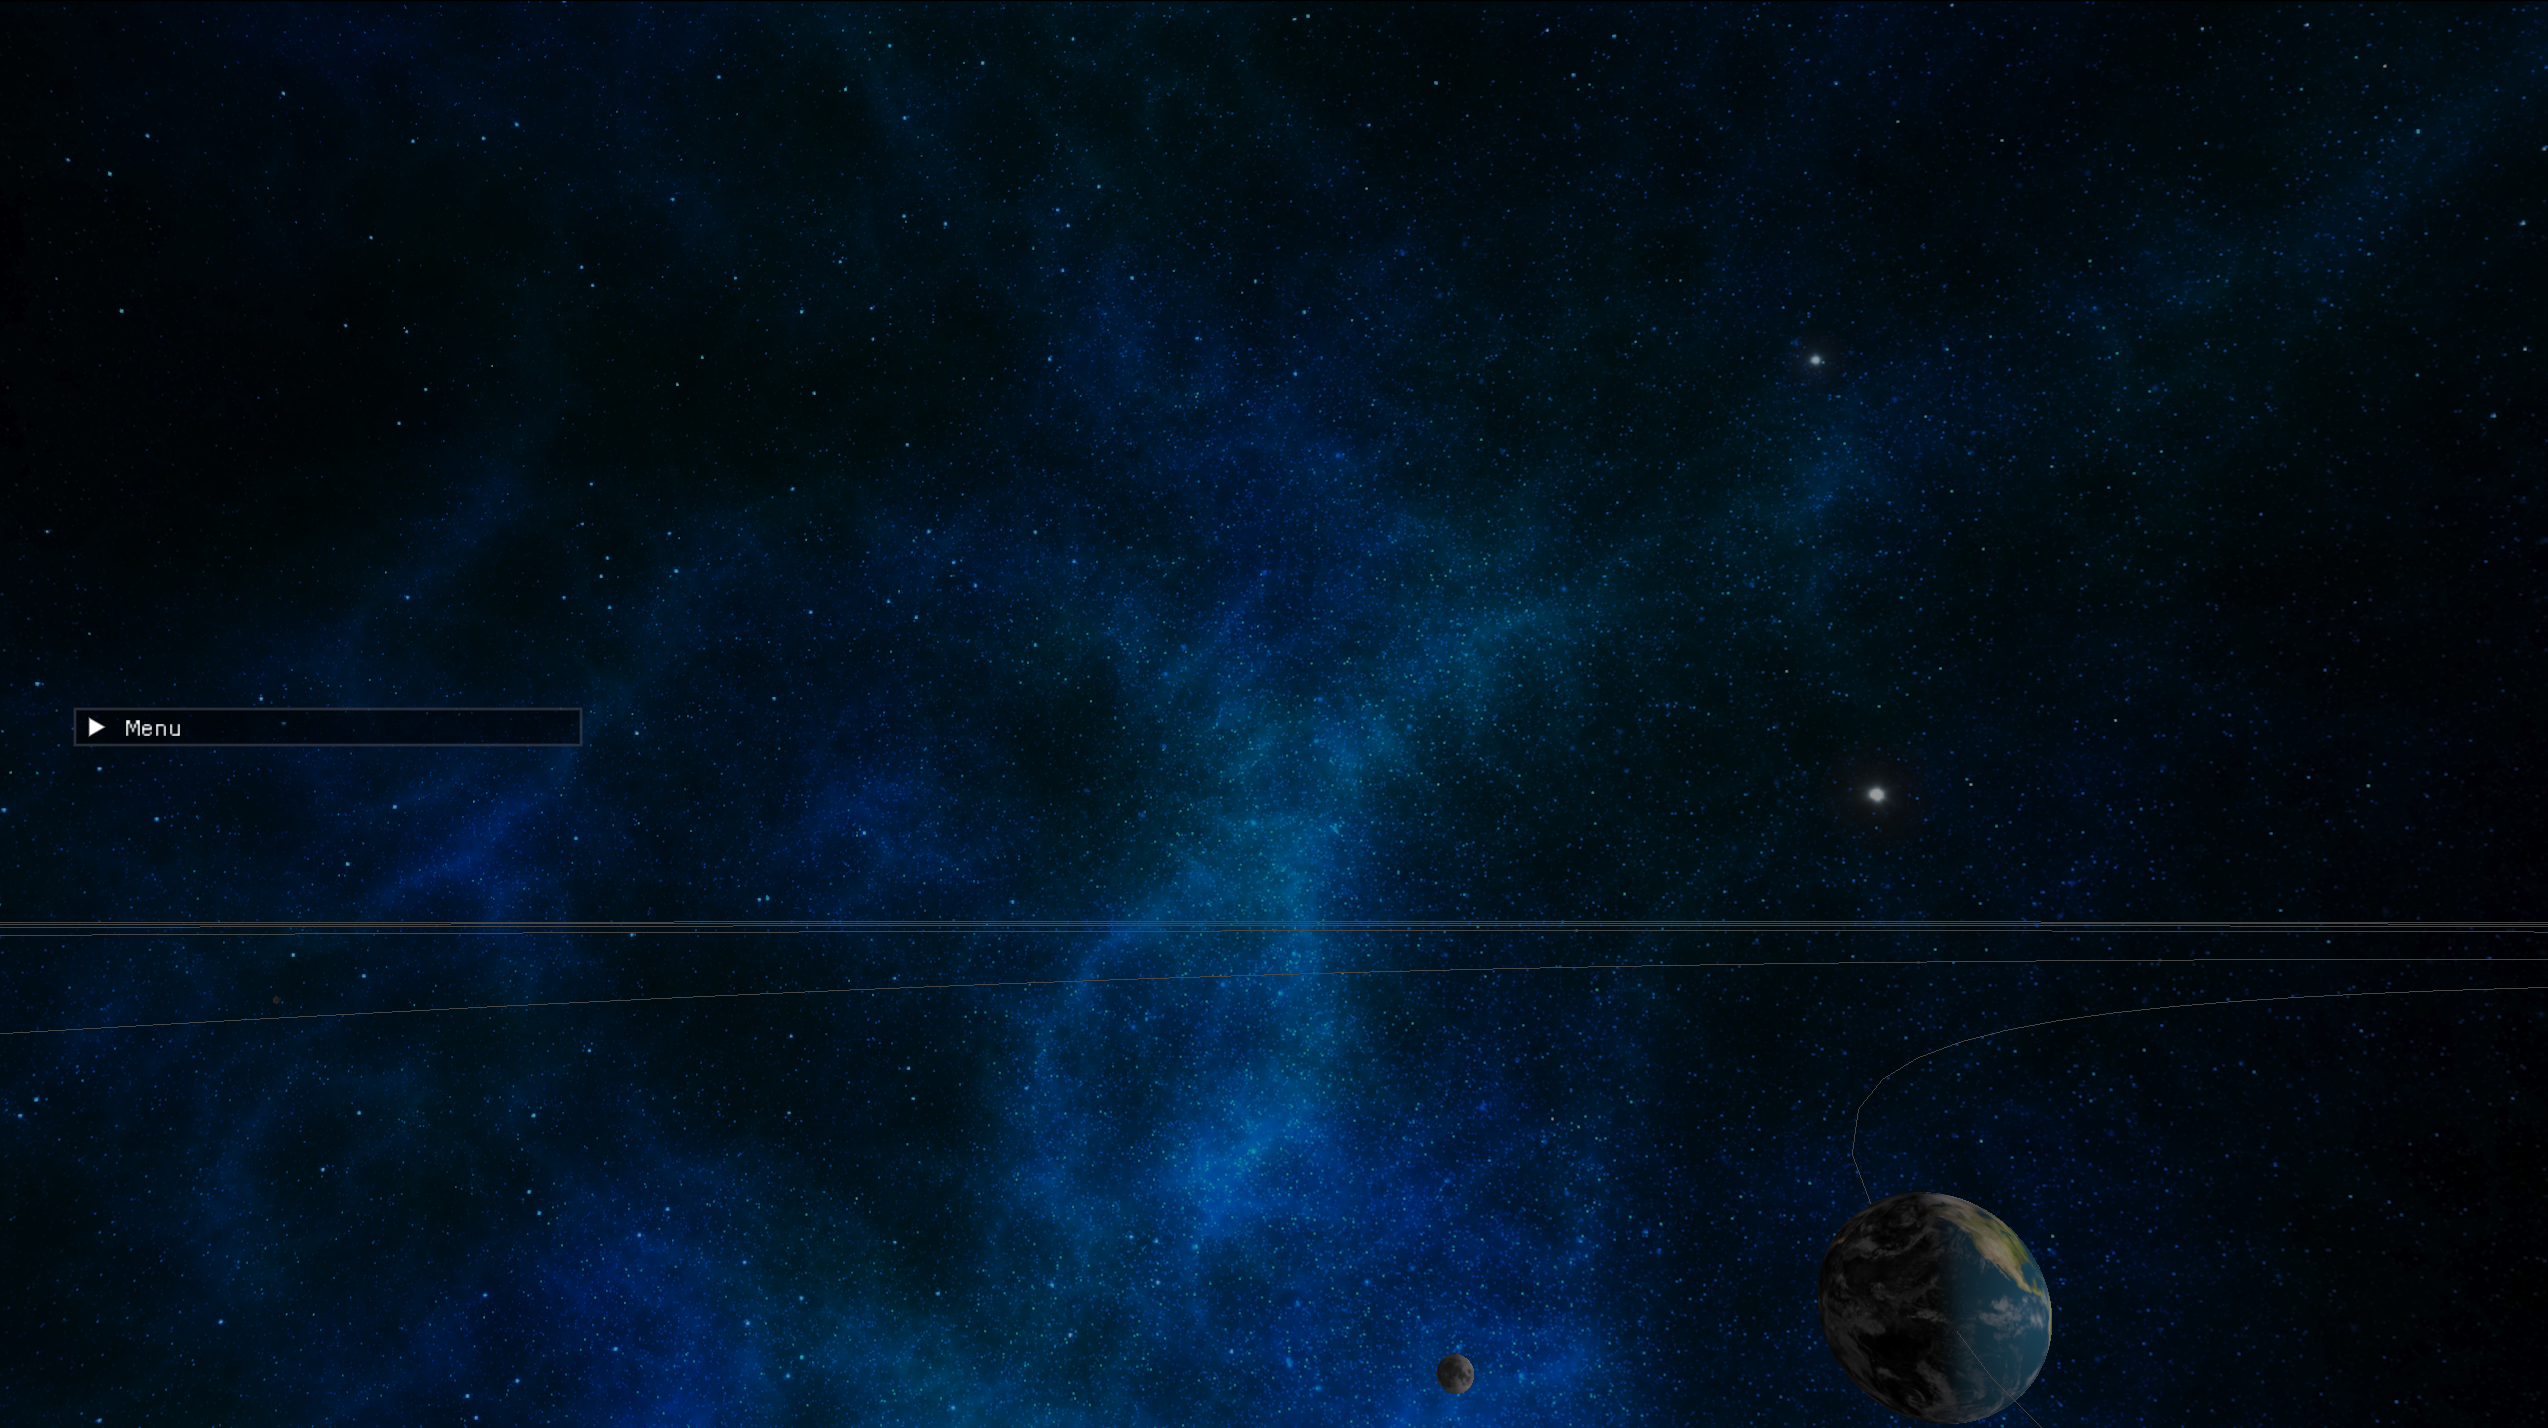
\includegraphics[width=200pt]{background.png}
    \caption{\textit{Skybox}}
\end{figure}

\subsection{\textit{Post-processing}}

Para as técnicas de \textit{Post-processing} que vamos explicar a seguir tivemos que adicionar algumas coisas à nossa simulação:
\begin{enumerate}
    \item \textit{Framebuffer}: O \textit{framebuffer} é uma porção da \ac{RAM} onde o \textit{OpenGL} armazena os pixeis que vão ser escritos no ecrã, ou seja, se tivermos acesso a ele podemos mudar os pixeis para obter os efeitos que desejamos (\textit{Post-processing}). Como o \textit{framebuffer} padrão do \textit{OpenGL} não é manipulável, criámos um onde renderizamos a nossa cena, aplicamos os efeitos, e escrevemos no mesmo um retângulo do tamanho do nosso \textit{display}.
    
    \item  \ac{HDR}: Por defeito os valores de cor dos pixeis no \textit{framebuffer} estao limitados entre 0.0 e 1.0, isso faz com que os pixeis com muito brilho percam definição por estarem limitados a 1.0. Ao passarmos o nosso \textit{framebuffer} de \texttt{GL\_RGB} para \texttt{GL\_RGBA16F}, obtemos pixeis com muita mais capacidade de representação dessa gama que antes estaria cortada. 
    No entanto, normalmente os nossos \textit{displays} são \ac{LDR}, por esse motivo têm essas mesmas limitações de cor e o resultado vai ser igual, mesmo tendo mais informação para representar os pixeis. Para mudar isto, precisamos de fazer o chamado \textit{Tone-mapping}.

    \item \textit{Tone-mapping}: É o processo de transformar números de precisão \textit{float} no limite [0.0; 1.0] esperado sem perder muito detalhe. Para usar este processo decidimos usar uma implementação com \textit{exposure} e \textit{gamma correction}.
\end{enumerate}

\newpage
\begin{lstlisting}[style=Cpp, caption=\textit{Fragment Shader} do \textit{framebuffer} para a \textit{exposure}]
void main() {
  ...
  const float adjSpeed = 0.05;
  float targetExposure = 0.5 / lum * 3.0f; 
  float sceneExposure = mix(exposure, targetExposure, adjSpeed);

  sceneExposure = clamp(exposure, 0.3f, 3.0f);

  vec3 mapped = vec3(1.0) - exp(-col * sceneExposure);
  mapped = pow(mapped, vec3(1.0 / gamma));
  ...
}
\end{lstlisting}

\subsection{\textit{Bloom}}
\label{chap2:sec:bloom}

\noindent
O \textit{bloom} é um efeito que nos permite dar o efeito de uma luz muito brilhante numa cena, algo que é dificíl de passar ao visualizador pelas limitações de cor anteriormente faladas.
A ideia é extraír as partes mais brilhantes da cena, desfocá-las, e combinar esse resultado com a imagem original.

\begin{figure}[h]
\centering
\includegraphics[width=450pt]{bloom_steps.png}
\caption{Passos do \textit{Bloom}}
\end{figure}

\newpage

\noindent
Como temos a nossa imagem em \ac{HDR}, podemos extraír as partes brilhantes da imagem facilmente:

\begin{lstlisting}[style=Cpp, caption=\textit{Fragment shader} do \textit{bloom}]
// lamp.frag
layout (location = 0) out vec4 FragColor;
layout (location = 1) out vec4 BrightColor;
...
void main() {
  color = texture(texture_diffuse, TexCoords) * sunIntensity;
  FragColor = color;

  float brightness = dot(color.rgb, vec3(0.2126, 0.7152, 0.0722));
  if(brightness > 1.0)
    BrightColor = vec4(color.rgb, 1.0);
  else
    BrightColor = vec4(0.0, 0.0, 0.0, 1.0);
}
\end{lstlisting}

\noindent
Para armazenarmos essa imagem nova, temos de informar o \textit{OpenGL} que queremos escrever em dois \textit{colorbuffers} no nosso \textit{framebuffer}:

\begin{lstlisting}[style=Cpp, caption=Escrita em 2 \textit{colorbuffers} diferentes]
void system() 
  ...
  unsigned int textureColorbuffer;
  glGenTextures(1, &textureColorbuffer);
  glBindTexture(GL_TEXTURE_2D, textureColorbuffer);
  glTexImage2D(GL_TEXTURE_2D, 0, GL_RGBA16F, SCREEN_WIDTH, SCREEN_HEIGHT, 0,
               GL_RGB, GL_FLOAT, NULL);
  glTexParameteri(GL_TEXTURE_2D, GL_TEXTURE_MIN_FILTER, GL_LINEAR);
  glTexParameteri(GL_TEXTURE_2D, GL_TEXTURE_MAG_FILTER, GL_LINEAR);
  glFramebufferTexture2D(GL_FRAMEBUFFER, GL_COLOR_ATTACHMENT0, GL_TEXTURE_2D,
                         textureColorbuffer, 0);

  unsigned int bloomTexture;
  glGenTextures(1, &bloomTexture);
  glBindTexture(GL_TEXTURE_2D, bloomTexture);
  glTexImage2D(GL_TEXTURE_2D, 0, GL_RGBA16F, SCREEN_WIDTH, SCREEN_HEIGHT, 0,
               GL_RGB, GL_FLOAT, NULL);
  glTexParameteri(GL_TEXTURE_2D, GL_TEXTURE_MIN_FILTER, GL_LINEAR);
  glTexParameteri(GL_TEXTURE_2D, GL_TEXTURE_MAG_FILTER, GL_LINEAR);
  glFramebufferTexture2D(GL_FRAMEBUFFER, GL_COLOR_ATTACHMENT1, GL_TEXTURE_2D,
                         bloomTexture, 0);

  ...

  unsigned int attachments[2] = {GL_COLOR_ATTACHMENT0, GL_COLOR_ATTACHMENT1};
  glDrawBuffers(2, attachments);
  ...
}
\end{lstlisting}

\noindent
A nossa imagem com pontos brilhantes passa assim a estar no \texttt{GL\_COLOR\_ATTACHMENT1} e a imagem original no \texttt{GL\_COLOR\_ATTACHMENT0}.  
O \textit{FragColor} no \textit{shader} anterior está a ser escrito no \texttt{GL\_COLOR\_ATTACHMENT0} e, por isso, na textura \textit{textureColorbuffer} enquanto o \textit{BrightColor} está a ser escrito no \texttt{GL\_COLOR\_ATTACHMENT1} e, por isso, na textura \textit{bloomTexture}.

\noindent
Aplicamos de seguida um filtro de \textbf{desfocagem Gaussiana}, que consiste em desfocar horizontalmente e depois verticalmente várias vezes seguidas, com pesos diferentes a cada iteração.
Feito isto combinamos os \textit{colorbuffers} \textbf{zero} e \textbf{um}, que são passados como texturas no \textit{Fragment Shader} do nosso \textit{framebuffer} e temos o efeito desejado.

\begin{lstlisting}[style=Cpp, caption=\textit{Fragment shader} do \textit{framebuffer}]
// framebuffer.frag
uniform sampler2D screenTexture;
uniform sampler2D bloomBlur;

...

void main() {
  vec3 col = texture(screenTexture, TexCoords).rgb;
  vec4 bloomTex = texture(bloomBlur, TexCoords);
  vec3 bloomColor = bloomTex.rgb;

  if (bloomActive)
    col += bloomColor;

  ...
}
\end{lstlisting}

\newpage
\subsection{\textit{Lens Flare}}

Um \textit{lens flare} é um efeito físico das câmeras reais que acontece quando uma luz intensa atinge o sistema de lentes de vidro que constituí a câmera. Este efeito estilístico faz com que a simulação pareça mais real, pois parece que estamos a ver algo gravado numa câmera verdadeira.

\noindent
O \textit{lens flare} é calculado em \textit{real-time} e não usa nenhuma textura convencional, apenas uma combinação de circulos com aberração cromática, junto de uma textura de ruído para um efeito mais aleatório.  

\noindent
A \textit{shader} usada foi adaptada \hyperlink{https://www.shadertoy.com/view/4sX3Rs}{deste \textit{lens flare}} \cite{shadertoy}.

\noindent
Para conseguir o efeito em que o \textit{lens flare} é obstruído por um planeta a passar entre a câmera e o sol, usámos o seguinte método:
\begin{enumerate}
    \item Criar uma \textit{hitbox} para cada planeta.
    \item Fazer um \textit{ray-cast} desde a câmera até ao centro do sol.
    \item Se este raio intercetar algum planeta, o \textit{lens flare} é desligado.
    \item Quanto mais longe o planeta estiver da câmera, menor será o seu raio de interseção.
\end{enumerate}

\begin{lstlisting}[style=Cpp, caption=Verificação da interseção do \textit{ray-cast}]
bool isIntersecting(glm::vec3 rayOrigin, glm::vec3 rayDirection,
                    const Sphere &sphere, float correction = 1.0f) {

  float cameraToPlanetLength = glm::length(sphere.center - camera.Position);
  float cutoff = cameraToPlanetLength / AU * correction;
  glm::vec3 oc = rayOrigin - sphere.center;
  float a = glm::dot(rayDirection, rayDirection);
  float b = 2.0f * glm::dot(oc, rayDirection);
  float c = glm::dot(oc, oc) -
            (glm::clamp(sphere.radius - cutoff, 0.0f, sphere.radius)) *
                (glm::clamp(sphere.radius - cutoff, 0.0f, sphere.radius));
  float discriminant = b * b - 4 * a * c;

  if (discriminant > 0) {
    float t1 = (-b - sqrt(discriminant)) / (2.0f * a);
    float t2 = (-b + sqrt(discriminant)) / (2.0f * a);

    if ((t1 >= 0.0f) || (t2 >= 0.0f)) {
      return true;
    }
  }
  return false;
}

...
void system() {
  ...
  while(!glfwWindowShouldClose()) {
    ...
    glm::vec3 rayDirection = glm::normalize(sunSphere.center - camera.Position);
    float rayLength = glm::length(sunSphere.center - camera.Position);
    glm::vec3 rayEndPoint = camera.Position + rayDirection * rayLength;
    if (lensFlareActive) {
      bool sunVisible =
          !isIntersecting(camera.Position, rayDirection, mercurySphere,
                          10.0f) &&
          !isIntersecting(camera.Position, rayDirection, venusSphere, 2.0f) &&
          !isIntersecting(camera.Position, rayDirection, earthSphere, 2.0f) &&
          !isIntersecting(camera.Position, rayDirection, marsSphere) &&
          !isIntersecting(camera.Position, rayDirection, jupiterSphere, 1.5f) &&
          !isIntersecting(camera.Position, rayDirection, saturnSphere) &&
          !isIntersecting(camera.Position, rayDirection, uranusSphere) &&
          !isIntersecting(camera.Position, rayDirection, neptuneSphere);
      screenShader.setBool("sunVisibleAndEnabled", sunVisible);
    } else {
      screenShader.setBool("sunVisibleAndEnabled", false);
    }
    ...
  }
  ...
}
\end{lstlisting}

\subsection{Música de Fundo}
\label{chap2:sec:musica}

\noindent
Foi usada a biblioteca \textbf{\textit{soloud}}, que nos permitiu facilmente adicionar música à nossa simulação. Há uma \textit{thread} dedicada para esse efeito.

\begin{lstlisting}[style=Cpp, caption=\textit{Thread} da Música]
std::thread audioThread(&initializeMiniaudio);
\end{lstlisting}

\noindent
Três sons são escolhidos aleatoriamente ao iniciar o sistema. Podemos trocar os mesmos por via do menu principal, e baixar ou aumentar o seu volume.

\newpage
\section{Conclusão}
\label{chap2:sec:concs}

\noindent
Concluimos assim a implementação da nossa simulação do sistema solar. Consideramos ter um sistema completo, tendo a terra com a sua lua, muitos asteróides espalhados, fundo no universo, luz solar que atinge a câmera e permite gerar um efeito mais realista e tendo também vários menus que permitem manipular o sistema em tempo de execução e ler informações sobre os diversos planetas.


\emptypage
\chapter{Conclusões e Trabalho Futuro}
\label{chap:conc-trab-futuro}

\section{Conclusões Principais}
\label{sec:conc-princ}

Dando por terminado o desenvolvimento deste projeto, concluímos que conseguimos alcançar todos os nossos objetivos, obtendo assim uma simulação realista do nosso sistema solar. Refletindo sobre tudo o que foi feito ao longo destes meses de trabalho, percebemos o quão importante é a área da \ac{CG} e o quão importante foi este projeto para a nosso aprendizagem, já que com ele conseguimos aprender muito para além do que foi possível nas aulas.
Concluímos também que fizémos um excelente trabalho, com uma boa organização e divisão do trabalho entre todos os elementos do grupo, estando muito orgulhosos do resultado final.

\section{Trabalho Futuro}
\label{sec:trab-futuro}

Neste projeto, devido a problemas de falta de tempo livre para investirmos mais no projeto, acabámos por não ter tempo para realizar a renderização de texto com auxílio de \textit{bitmaps} ou \textit{billboards}, mas ficando assim como um objetivo futuro para aprimoramento do projeto. Para suprir a falta disto, criámos labels por via de menus com ajuda da biblioteca \ac{IMGUI}.

\noindent
Para além disso, seria bastante interessante adicionar à nossa simulação outros planetas e galáxias distantes, ou até mesmo simular buracos negros e "brincar" com a gravidade e todas as leis da física que conhecemos hoje.

\emptypage
\backmatter

\bibliographystyle{unsrt}
\bibliography{bibliografia}

\end{document}
